\documentclass{beamer}
\usepackage{ragged2e}
\usepackage{amsmath,amssymb}

\title{Modelos Generativos Profundos}
\subtitle{Clase 13: Redes generativas adversarias (parte II)}
\author{Fernando Fêtis Riquelme}
\institute{
    Facultad de Ciencias Físicas y Matemáticas\\
    Universidad de Chile
}
\date{Otoño, 2026}
\titlegraphic{\hfill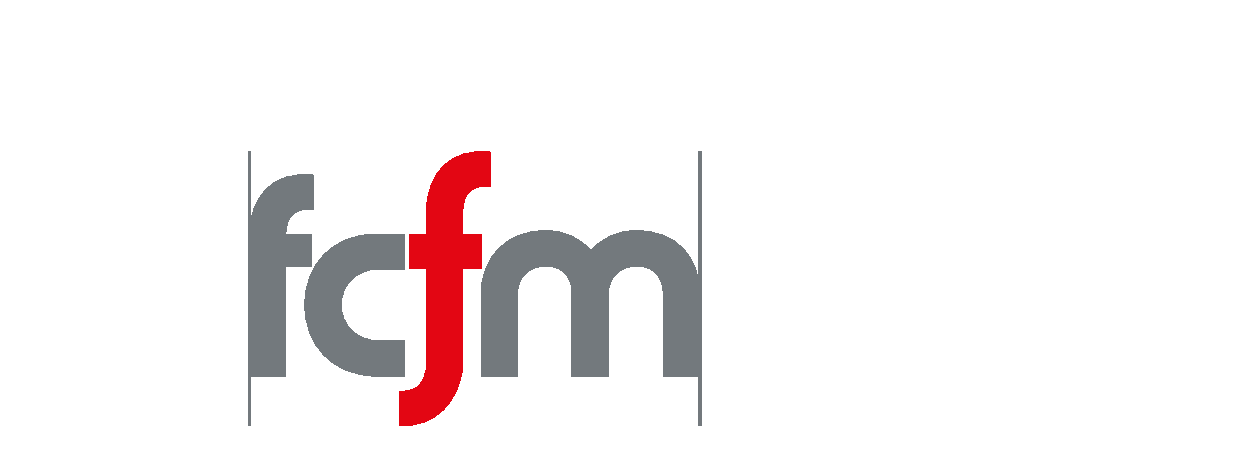
\includegraphics[height=1.2cm]{images/fcfm}}

\usetheme{metropolis}

\newcommand{\R}{\mathbb{R}}
\newcommand{\N}{\mathbb{N}}
\newcommand{\Z}{\mathbb{Z}}
\newcommand{\argmax}{\operatorname{argmax}}
\newcommand{\argmin}{\operatorname{argmin}}
\newcommand{\insertimage}[2]{
    \begin{center}
        \includegraphics[width=#2\textwidth]{images/#1}
    \end{center}
}
\setlength{\leftmargini}{0em}
\renewcommand{\raggedright}{\leftskip=0pt \rightskip=0pt plus 0cm}

\setbeamercovered{invisible}

\justifying

\begin{document}

\begin{frame}
    \titlepage
\end{frame}

\begin{frame}{Clase de hoy}
    \tableofcontents
\end{frame}

\section{Recuerdo clase anterior}

\begin{frame}{Idea general}
    Una GAN es un modelo de variable latente, $p_\theta(x,z)=p(z)p_\theta(x|z)$ con $p(z)=\mathcal{N}(0,\mathrm{I}_L)$ y $p_\theta(x|z)=\delta_{G_\theta(z)}(x)$, donde $G_\theta:\R^L\to\R^D$ es una red neuronal.

    La red generadora $G_\theta$ es entrenada para engañar a un discriminador $q_\phi(y| x)\sim\text{Bernoulli}(D_\phi(x))$, con $D_\phi:\R^D\to[0,1]$ una red neuronal, el cual a su vez aprende a diferenciar muestras provenientes de $p_\text{data}(x)$ ($y=1$) o de $p_\theta(x)$ ($y=0$).
\end{frame}

\begin{frame}{Función objetivo}
    Si el clasificador $q_\phi(y|x)$ es optimizado mediante máxima verosimilitud, entonces una GAN se reduce al siguiente juego:
    \begin{equation*}
        \min_\theta \max_\phi\mathbb{E}_{p_\text{data}(x)}\left[\log D_\phi(x)\right] + \mathbb{E}_{z\sim\mathcal{N}(0,\mathrm{I}_L)}\left[\log(1-D_\phi(G_\theta(z)))\right]
    \end{equation*}
    En la práctica, se suele utilizar una versión no saturante en el generador, llegando a las siguientes funciones de pérdida:
    \begin{align*}
        \mathcal{L}_D(\phi)   & = -\mathbb{E}_{p_\text{data}(x)}\left[\log D_\phi(x)\right] - \mathbb{E}_{z\sim\mathcal{N}(0,\mathrm{I}_L)}\left[\log(1-D_\phi(G_\theta(z)))\right] \\
        \mathcal{L}_G(\theta) & = -\mathbb{E}_{z\sim\mathcal{N}(0,\mathrm{I}_L)}\left[\log D_\phi(G_\theta(z))\right].
    \end{align*}
\end{frame}

\section{Convolución transpuesta}

\begin{frame}{Motivación CNN}
    Las redes convolucionales permiten inducir un sesgo de \textbf{localidad} e \textbf{invarianza a traslaciones} de features dentro de la entrada, lo que las vuelve útiles para el diseño de arquitecturas neuronales para imágenes.

    Por otro lado, dada la dificultad de entrenar una GAN, es necesario utilizar arquitecturas específicas que permitan estabilizar el entrenamiento y obtener buenos resultados.

    Si bien muchas de estas heurísticas son solo empíricas, varias de ellas siguen siendo importantes en la actualidad.
\end{frame}

\begin{frame}{Motivación CNN transpuestas}
    Por otro lado, una convolución estándar suele reducir la dimensión de entrada de la imagen (o en el mejor de los casos, mantenerla).

    En una GAN se suele comenzar con una representación latente de baja dimensión, la cual va aumentando progresivamente a medida que se avanza en la red neuronal.

    La convolución transpuesta es una operación dual que permite aumentar la dimensión de la entrada, lo que la hace útil para el diseño de arquitecturas de generadores en GANs.
\end{frame}

\begin{frame}{Convolución como operador lineal}
    Dada una entrada $x\in\R^{D_\text{in}}$, una \textbf{convolución} con \textbf{filtro} $w\in\R^K$, \textbf{stride} $S\geq1$ y \textbf{padding} $P\geq0$ produce una salida $y\in\R^{D_\text{out}}$ con
    \begin{equation*}
        y_d = \sum_{k=1}^K w_k\,x_{S(d-1)+k-P}, \qquad d=1,\ldots,D_\text{out},
    \end{equation*}
    donde $x_d=0$ para $d\notin\{1,\ldots,D_\text{in}\}$ (zero-padding implícito) y
    \begin{equation*}
        D_\text{out} = \left\lfloor\frac{D_\text{in}+2P-K}{S}\right\rfloor + 1.
    \end{equation*}
    Notar que esta operación se puede escribir como $y=Ax$, donde $A\in\mathcal{M}_{D_\text{out},D_\text{in}}(\R)$ es una \textbf{matriz de Toeplitz}. En particular, la convolución es una transformación lineal.
\end{frame}

\begin{frame}{Convolución como operador lineal}
    La siguiente imagen muestra una convolución 2D con hiperparámetros $K=3$, $P=1$ y $S=2$:
    \insertimage{conv}{0.8}
\end{frame}

\begin{frame}{Convolución transpuesta}
    Dada una convolución con matriz $A\in\mathcal{M}_{D_\text{out},D_\text{in}}(\R)$, la \textbf{convolución transpuesta} es el operador $A^\top:\R^{D_\text{out}}\to\R^{D_\text{in}}$:
    \begin{itemize}
        \item En particular, si $D_\text{out}<D_\text{in}$ (como en una convolución estándar), la convolución transpuesta aumenta la dimensión de la entrada.
        \item Más precisamente, el tamaño de la salida de una convolución transpuesta con entrada $y\in\R^{D_\text{out}}$ es:
              \begin{equation*}
                  D_\text{in} = S(D_\text{out}-1) + K - 2P.
              \end{equation*}
    \end{itemize}
    En particular, el caso estándar $K=4$, $S=2$, $P=1$ duplica la dimensión de salida ($D_\text{in}=2D_\text{out}$).
\end{frame}

\begin{frame}{Convolución transpuesta}
    En la práctica, la convolución transpuesta es equivalente a intercalar $S{-}1$ ceros entre los elementos de la entrada y aplicar una convolución estándar con stride 1.

    Esto motiva a llamar a la convolución transpuesta convolución con \textbf{stride fraccionario}.

    Por otro lado, la convolución y la convolución transpuesta 1D se puede extender a varias dimensiones aplicándola por separado en cada dimensión, con sus propios hiperparámetros $K$, $S$ y $P$.
\end{frame}

\begin{frame}{Convolución transpuesta}
    La siguiente imagen muestra una convolución transpuesta 2D con hiperparámetros $K=3$, $P=1$ y $S=2$:
    \insertimage{tconv}{1}
\end{frame}

\begin{frame}{Checkerboard artifact}
    En una convolución transpuesta, si $S$ no es múltiplo de $K$, cada posición de la salida recibirá un número desigual de contribuciones del filtro, produciendo un patrón periódico en la imagen generada.

    Existen dos estrategias para evitar este fenómeno:
    \begin{enumerate}
        \item Elegir $K=2S$, de modo que todas las posiciones reciban el mismo número de contribuciones.
        \item Realizar interpolación clásica (e.g. upsampling bilineal o nearest-neighbor) seguido de una convolución estándar.
    \end{enumerate}
\end{frame}

\begin{frame}{Checkerboard artifact}
    \insertimage{checkboard_1}{1}
\end{frame}

\begin{frame}{Checkerboard artifact}
    \insertimage{checkboard_2}{1}
\end{frame}

\section{DCGAN}

\begin{frame}{Deep convolutional GAN}
    \textbf{DCGAN} fue uno de los primeros trabajos en obtener buenos resultados a resolución $64\times64$.

    Este trabajo estableció empíricamente algunos principios básicos para el diseño de arquitecturas de GANs para imágenes:
    \begin{enumerate}\textbf{}
        \item Usar arquitecturas \textbf{completamente convolucionales}.
        \item \textbf{Batch normalization} en todas las capas, excepto en la salida de $G_\theta$ y la entrada de $D_\phi$.
        \item Convoluciones con stride en lugar de pooling.
        \item Activaciones ReLU en $G_\theta$ y LeakyReLU en $D_\phi$.
        \item Activación $\tanh$ en la salida de $G_\theta$.
        \item Durante la optimizacion, usar Adam con $\beta_1=0.5$.
    \end{enumerate}
\end{frame}

\begin{frame}{Propiedades del espacio latente}
    Un resultado relevante de DCGAN fue verificar que el espacio latente de una GAN permite realizar \textbf{interpolación semántica}.

    Dadas dos muestras latentes, $z^0,z^1\sim\mathcal{N}(0,\text{I}_L)$, la curva
    \begin{equation*}
        t\mapsto G_\theta\left((1-t)z_0+tz_1\right), \qquad t\in[0,1],
    \end{equation*}
    produce transiciones visuales suaves entre los atributos de las muestras $G_\theta(z_0)$ y $G_\theta(z_1)$.

    Más aún, DCGAN mostró que es posible realizar \textbf{aritmética vectorial} el espacio latente, pudiendo modificar atributos específicos de la imagen generada sumando o restando vectores latentes directores correspondientes a esos atributos.
\end{frame}

\begin{frame}{Propiedades del espacio latente}
    \insertimage{dcgan_1}{1}
\end{frame}

\begin{frame}{Propiedades del espacio latente}
    \insertimage{dcgan_2}{1}
\end{frame}

\section{SAGAN}

\begin{frame}{Self-attention GAN}
    Las CNNs suelen presentar dificultades para modelar dependencias de largo alcance debido a su naturaleza local.

    \textbf{SAGAN} propone incorporar considerar cada pixel $(x_1,\ldots,x_N)\subset\R^C$ (con $N=H\times W$) como un token y aplicar un módulo de self-attention que permita capturar dependencias entre cualquier par de posiciones del feature map con un único bloque:
    \begin{equation*}
        y_i = \gamma\left(W_O\sum_{j=1}^N a_{ij}\,(W_V x_j)\right) + x_i,
        \quad\text{donde}\quad
        a_{ij} = \frac{\exp\left({\langle W_Q x_i, W_K x_j\rangle}\right)}{\sum_{t} \exp\left({\langle W_Q x_i, W_K x_t\rangle}\right)}
    \end{equation*}

    El parámetro entrenable $\gamma\in\R$ se inicializa en $0$ para que la red comience como una CNN pura e incorpore dependencias de largo alcance gradualmente durante la optimización.
\end{frame}

\begin{frame}{Mapa de atención}
    \insertimage{sagan_attn}{1}
\end{frame}

\begin{frame}{Hinge adversarial loss}
    SAGAN también utiliza otras heurísticas de diseño como \textbf{normalización espectral} o \textbf{TTUR}, las cuales permiten ver la dificultad de entrenar GANs.

    Otro cambio usual en GANs es variar otra función de pérdida. En el caso de SAGAN, la \textbf{hinge adversarial loss} trata a $D_\phi$ como un margen de SVM:
    \begin{align*}
        \mathcal{L}_D(\phi)   & = -\mathbb{E}\!\left[\min(0,-1+D_\phi(x))\right] - \mathbb{E}\!\left[\min(0,-1-D_\phi(G_\theta(z)))\right] \\
        \mathcal{L}_G(\theta) & = -\mathbb{E}\!\left[D_\phi(G_\theta(z))\right],
    \end{align*}
    donde ahora $D_\phi(x)\in\R$ es un score de clasificación.
\end{frame}

\section{ProGAN}

\begin{frame}{Progressive GAN}
    \textbf{ProGAN} fue el primer método en producir imágenes convincentes a una resolución de$1024\times1024$.

    En este enfoque, $G_\theta$ y $D_\phi$ comienzan en una resolución de $4\times4$ y van agregando progresivamente pares de capas hasta la resolución objetivo (\textbf{curriculum learning}).

    Al igual que los trabajos anteriores, ProGAN también propone otro conjunto de heurísticas que pueden ayudar a estabilizar el entrenamiento.

    Entre ellas, está usar la pérdida de \textbf{Wasserstein GAN}, la cual relaciona directamente las GANs con transporte óptimo.
\end{frame}

\begin{frame}{Arquitectura}
    \insertimage{progan}{1}
\end{frame}

\begin{frame}{Fade-in}
    Para poder ampliar la resolución apilando más capas convolucionales, ProGAN utiliza dos convoluciones $1\times 1$ necesarias durante el entrenamiento:
    \begin{itemize}
        \item $\operatorname{toRGB}_r:\R^{C\times r\times r}\to\R^{3\times r\times r}$ (usada por el generador).
        \item $\operatorname{fromRGB}_r:\R^{3\times r\times r}\to\R^{C\times r\times r}$ (usada por el discriminador).
    \end{itemize}
    Con esto, durante la transición $r\to 2r$, para $\alpha\in[0,1]$ que aumenta linealmente durante el entrenamiento, se considera
    \begin{itemize}
        \item $G_\text{out} = (1-\alpha)\,\operatorname{toRGB}_{2r}\!\left(\operatorname{up}(h_r)\right) + \alpha\,\operatorname{toRGB}_{2r}\!\bigl(\operatorname{conv}(\operatorname{up}(h_r))\bigr)$.
        \item $D_\text{in} = (1-\alpha)\,\operatorname{fromRGB}_{r}\!\left(\operatorname{down}(x_{2r})\right) + \alpha\,\operatorname{fromRGB}_{2r}\!\bigl(\operatorname{conv}(\operatorname{down}(u_{2x}))\bigr)$.
    \end{itemize}
    donde $h_r$ es el feature map de $G_\theta$ en resolución $r\times r$ y $x_{2r}$ la imagen real en resolución $2r\times 2r$.
\end{frame}

\section{StyleGAN}

\begin{frame}{Idea general}
    Si bien ProGAN permite generar imágenes de alta calidad, no permite controlar fácilmente atributos específicos de la imagen generada, lo que limita su aplicabilidad.

    \textbf{StyleGAN} es una arquitectura de generador que permite desacoplar la distribución del espacio latente de la GAN para poder realizar un mejor control de los atributos de la imagen generada.

    Para esto, inyecta información de estilo en cada capa de la red mediante métodos de \textbf{modulación}.
\end{frame}

\begin{frame}{Arquitectura}
    \insertimage{stylegan_arch}{0.5}
\end{frame}

\begin{frame}{Mapping network}
    Para empezar, StyleGAN mapea la representación latente $z\in\R^L$ a una representación intermedia $w\in\R^L$ mediante una \textbf{mapping network} $f_\psi:\R^L\to\R^L$.

    La idea es que $f_\psi$ pueda aprender a transformar la distribución $p_\theta(z)\sim\mathcal{N}(0,\mathrm{I}_L)$ a una distribución más adecuada para el control de atributos en $w$.

    Esto es necesario ya que, sin esta red, $G_\theta$ debe doblarse para evitar generar muestras poco probables, lo que rompe la linealidad semántica del espacio latente.
\end{frame}

\begin{frame}{Synthesis network}
    La \textbf{synthesis network} $g_\omega:\R^L\to\R^{3\times H\times W}$ genera imágenes inyectando la representación intermedia $w$ en cada capa de la red utilizando \textbf{adaptative instance normalization (AdaIN)}:
    \begin{equation*}
        \operatorname{AdaIN}(x_c, w) = \alpha_c\,\frac{x_c-\mu(x_c)}{\sigma(x_c)} + \beta_c
        \in\R^{H\times W},
    \end{equation*}

    donde $x_c\in\R^{H\times W}$ es el $c$-ésimo canal de la capa, $\mu(x_c)$ y $\sigma(x_c)$ son su media y desviación estándar, y $(\alpha,\beta)\in\R^C\times\R^C$ provienen de una transformación afín aprendida, $A:\R^L\to\R^C\times\R^C$.

    De esta forma, la red comienza desde un tensor inicial $c_0\in\R^{C_0\times H_0\times W_0}$ y luego cada capa aplica AdaIN con un estilo específico definido por $w$.
\end{frame}

\begin{frame}{Style mixing}
    La técnica anterior permite controlar atributos específicos de la imagen generada, ya que cada capa de la red controla atributos de diferente nivel de abstracción.

    StyleGAN también realiza \textbf{style mixing}, donde se cruzan dos latentes $w_1$, $w_2$ en una capa $\ell^*$ aleatoria. En estos casos, capas de baja resolución controlan pose y estructura, mientras que capas de alta resolución controlan textura y detalles finos.
\end{frame}

\section{U-Net}

\begin{frame}{Arquitectura U-Net}
    Cuando la condición de una CGAN condicional es una imagen, es usual requerir una arquitectura que preserve la estructura espacial. La \textbf{U-Net} es un autoencoder completamente convolucional con \textbf{skip connections} entre encoder y decoder:
    \begin{itemize}
        \item El \textbf{encoder} reduce progresivamente la resolución extrayendo representaciones de alto nivel.
        \item El \textbf{decoder} recupera la resolución mediante upsampling y concatena, en cada nivel, la activación homóloga del encoder.
        \item Estas skip connections permiten transmitir directamente información espacial de bajo nivel desde el encoder hacia el decoder, sin pasar por el cuello de botella.
    \end{itemize}
\end{frame}

\begin{frame}{Arquitectura U-Net}
    \insertimage{unet}{1}
\end{frame}

\begin{frame}{Relevancia de la U-Net}
    En un comienzo, la U-Net fue propuesta para \textbf{segmentación semántica} (clasificación por píxel), pero su arquitectura se volvió muy popular para tareas de generación de imágenes:
    \begin{itemize}
        \item En GANs condicionales image-to-image (e.g., \textbf{pix2pix}), el generador suele ser una U-Net.
        \item En modelos de difusión, la U-Net modificada con mecanismos de atención permite generar imágenes de alta calidad y condicionar con respecto a texto.
    \end{itemize}
\end{frame}

\begin{frame}{Próxima clase}
    En la próxima clase:
    \begin{itemize}
        \item Transferencia de estilo.
        \item Nociones de transporte óptimo.
        \item Algunas cosas de las GANs.
    \end{itemize}
\end{frame}

\begin{frame}
    \centering
    \Large{Modelos Generativos Profundos}\\
    \large{Clase 13: Redes generativas adversarias (parte II)}
\end{frame}

\end{document}
